\documentclass[12pt]{article}

\usepackage[dvips,letterpaper,landscape]{geometry}
\usepackage[pdftex]{graphicx}
% \special{landscape}
% \usepackage[letterpaper,landscape]{geometry}

\textheight 6.5in

%opening
\title{AT Cases}
\date{}
% \author{}

\begin{document}

\maketitle


Here are the images I used at our meeting on Thursday. We did five
correlation tests, each of which was computed between the PFT values and
image metrics from

1. expiration of whole lung  --- ( *\_whole\_exp.jpg )

2. inspiration of whole lung --- ( *\_whole\_insp.jpg )

3. inspiration of whole lung minus expiration of whole lung --- (
*\_whole.jpg )

4. Jacobian from the registration --- ( *\_jac.jpg )

5. the PFT value themselves --- ( *\_self.jpg )

For each test, we computed the correlation value and the p test value
(using Matlab corrcoef). rho\_*.jpg shows the correlation value and
p\_*.jpg shows if the p value is smaller than 0.01 (yes if in red and no
if in blue).

One more clarification is about the 3rd test. This is correlated with (
the value from expiration image metrics - the value from inspiration
image metrics), not with the value from the differencing image of
inspiration and expiration.

Also, volume.jpg plots the FVC value and the value of  the segmentation
volume of inspiration subtracted by the one of expiration volume. This
plot shows the correlation from the left-top grid in *\_whole.jpg.


\begin{figure}
 % \centering
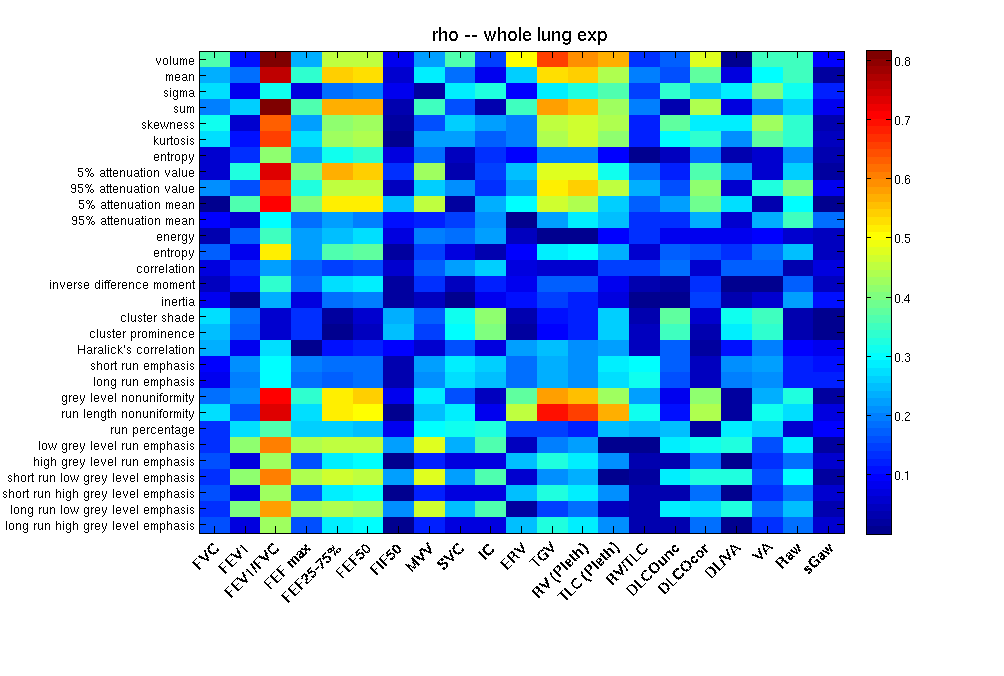
\includegraphics[width=0.9\linewidth,viewport=100 60 620 520]{rho_whole_exp.png}
% 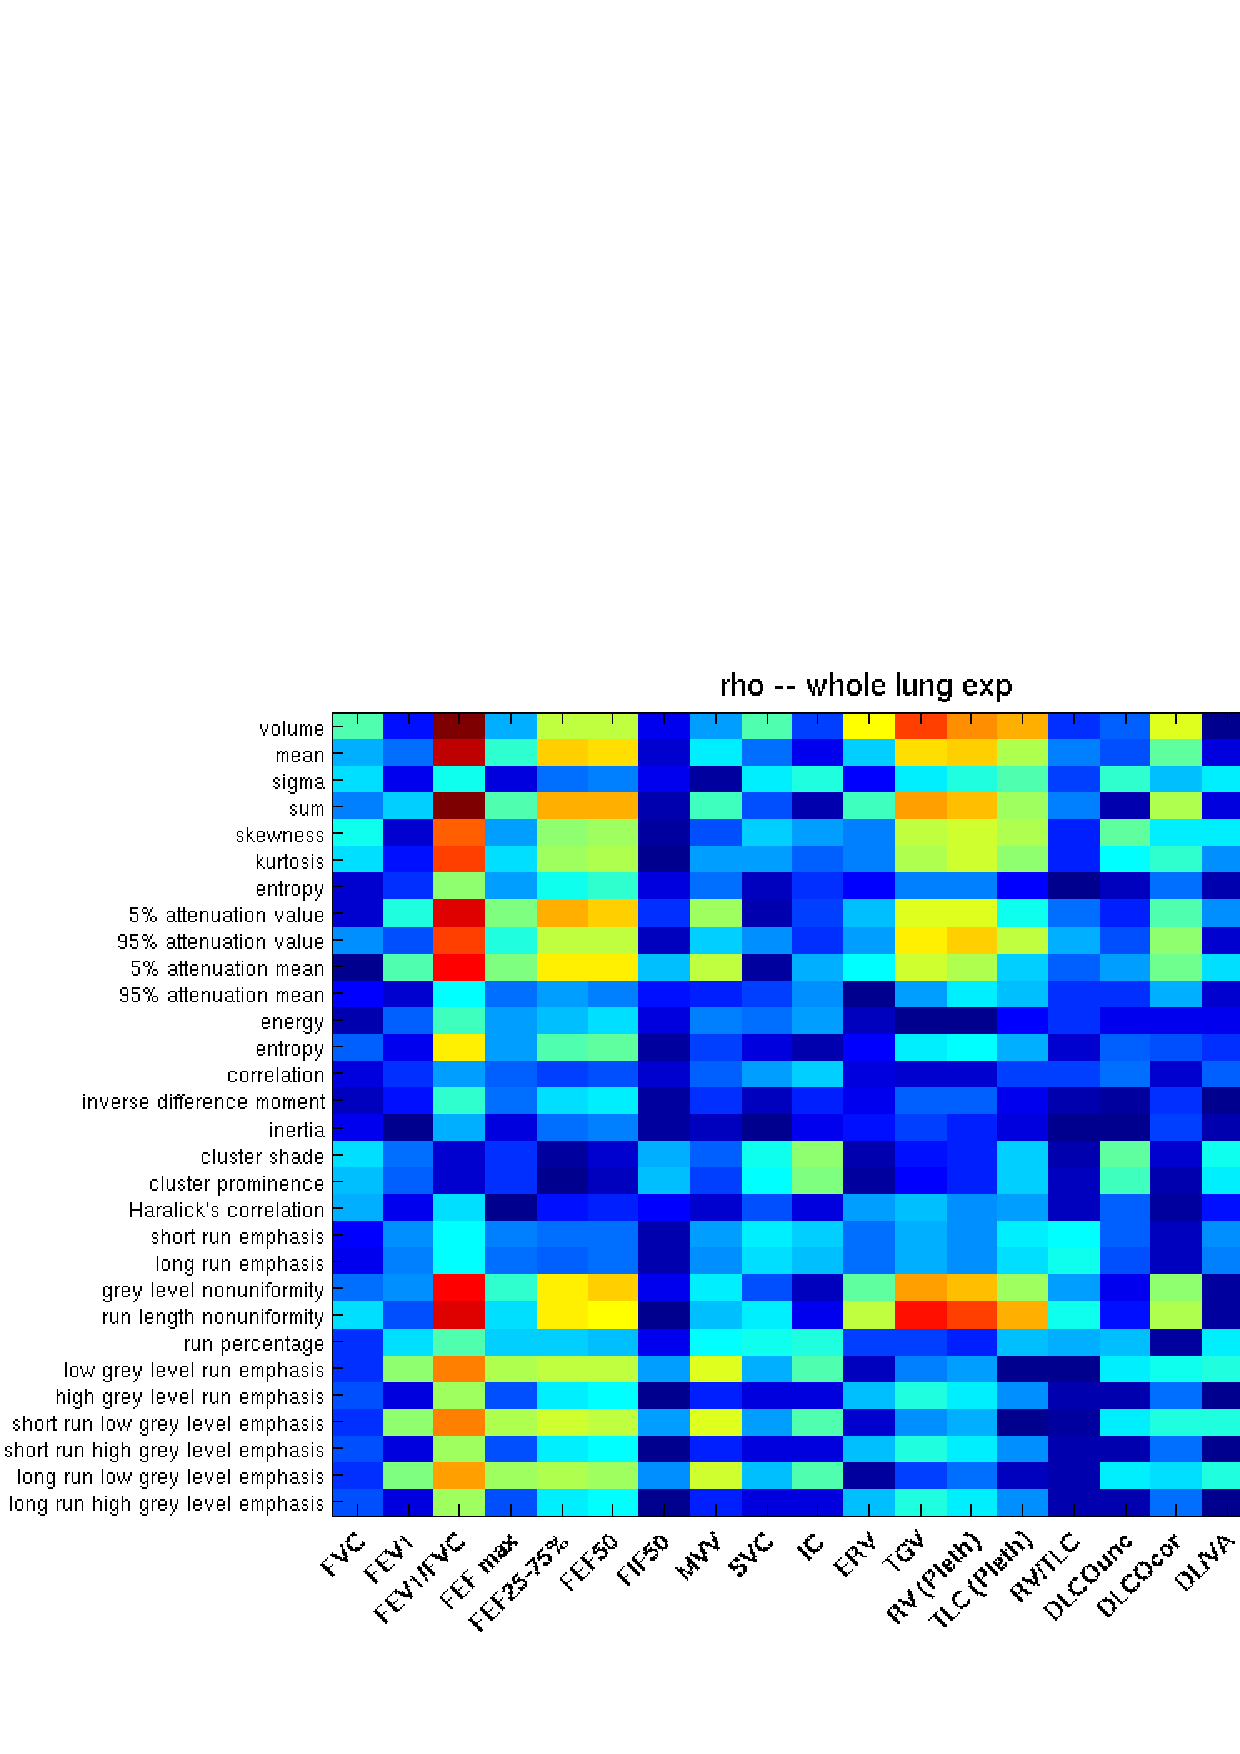
\includegraphics[width=0.9\linewidth,viewport=100 60 620 520]{rho.png}
 \caption{rho\_whole\_exp. PFT correlated with lung expiration, rho value.}
\end{figure}

\begin{figure}
 % \centering
 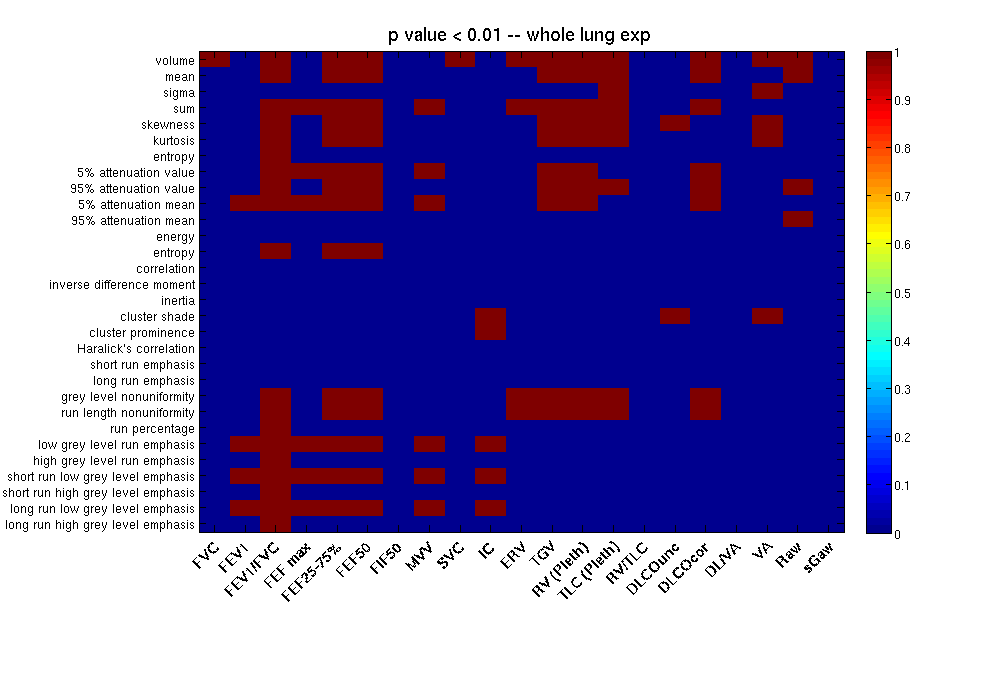
\includegraphics[width=0.9\linewidth,viewport=100 60 620 520]{p_whole_exp.png}
 \caption{p\_whole\_exp. PFT correlated with lung expiration, p value $<$ 0.01.}
\end{figure}

\begin{figure}
 % \centering
 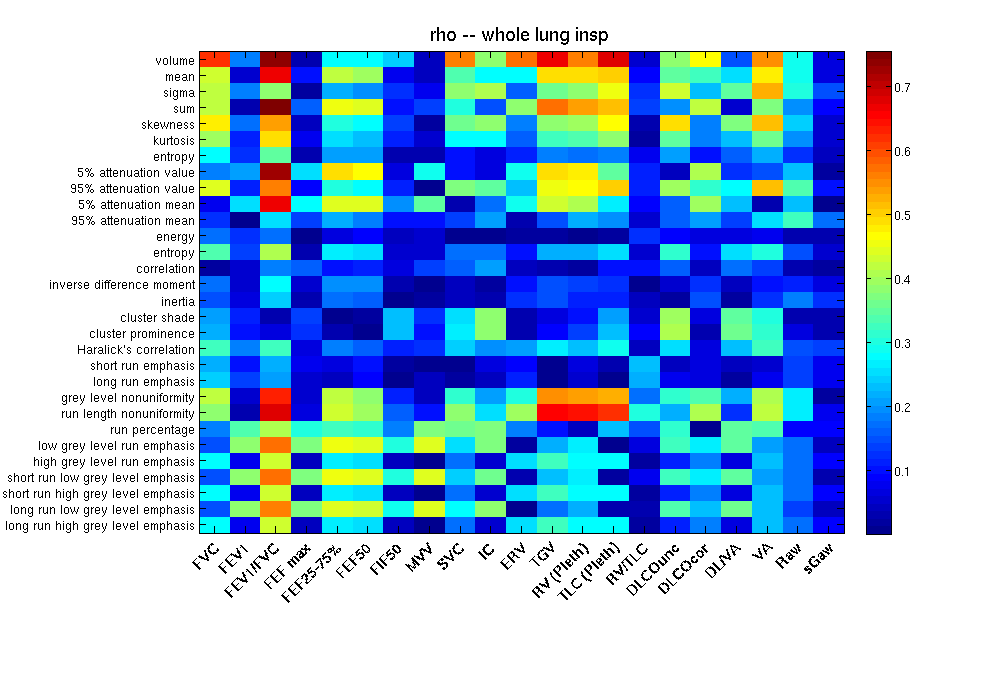
\includegraphics[width=0.9\linewidth,viewport=100 60 620 520]{rho_whole_insp.png}
 \caption{rho\_whole\_insp. PFT correlated with lung inspiration, rho value.}
\end{figure}

\begin{figure}
 % \centering
 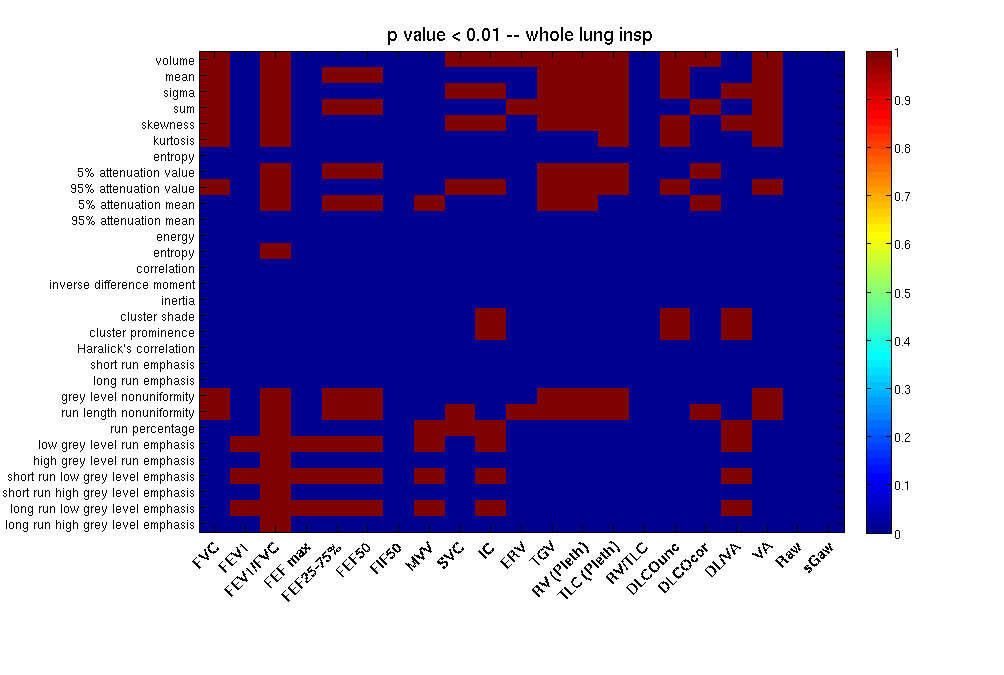
\includegraphics[width=0.9\linewidth,viewport=100 60 620 520]{p_whole_insp.png}
 \caption{p\_whole\_insp. PFT correlated with lung inspiration, p value $<$ 0.01.}
\end{figure}

\begin{figure}
 % \centering
 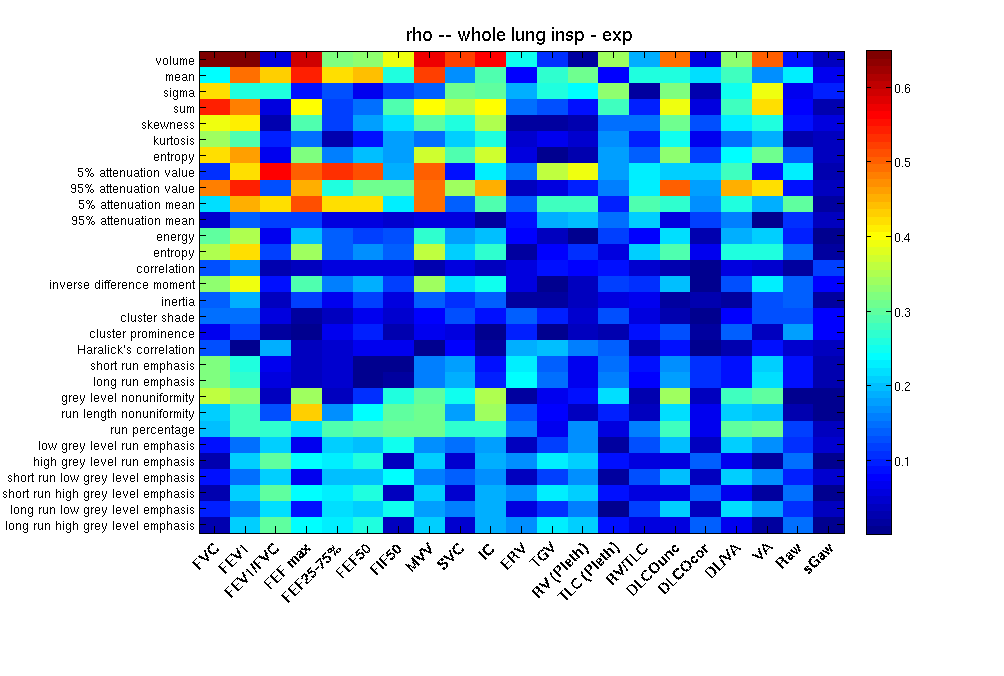
\includegraphics[width=0.9\linewidth,viewport=100 60 620 520]{rho_whole.png}
 \caption{rho\_whole. PFT correlated with lung inspiration metrics minus expiration metrics, rho value.}
\end{figure}

\begin{figure}
 % \centering
 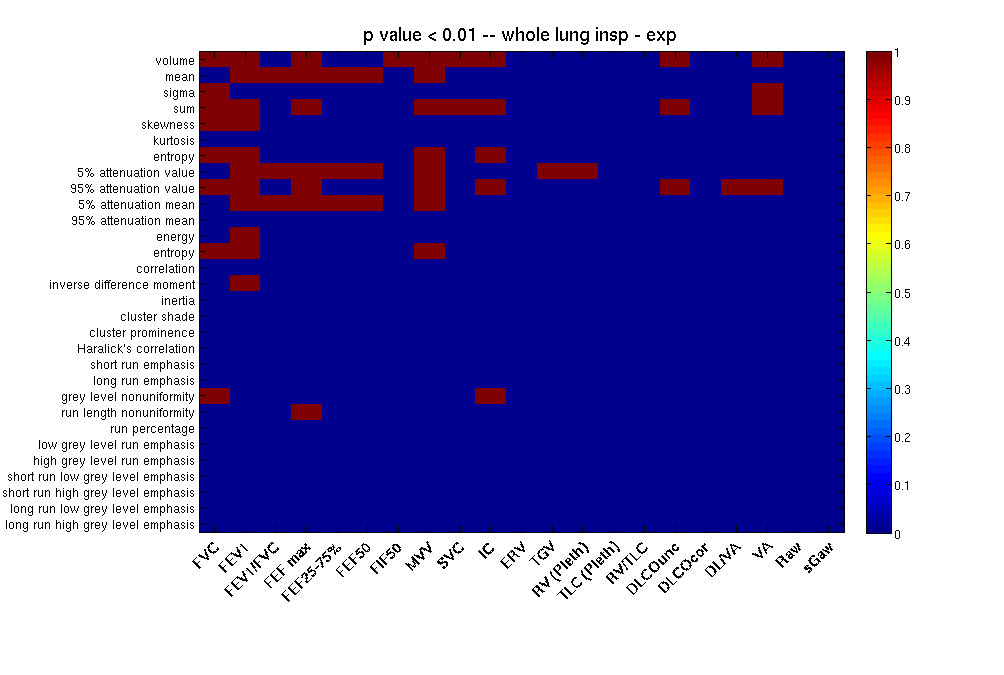
\includegraphics[width=0.9\linewidth,viewport=100 60 620 520]{p_whole.png}
 \caption{p\_whole. PFT correlated with lung inspiration metrics minus expiration metrics, p value $<$ 0.01.}
\end{figure}

\begin{figure}
 \centering
 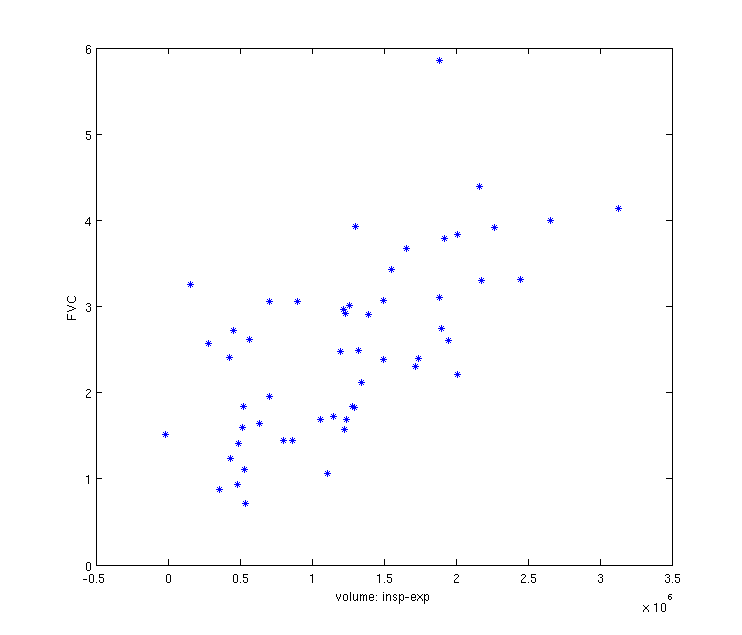
\includegraphics[width=0.8\linewidth,viewport=0 0 500 450]{volume.png}
 \caption{volume. FVC versus segmentation volum of lung inspiration minus volume of expiration.}
\end{figure}

\begin{figure}
 % \centering
 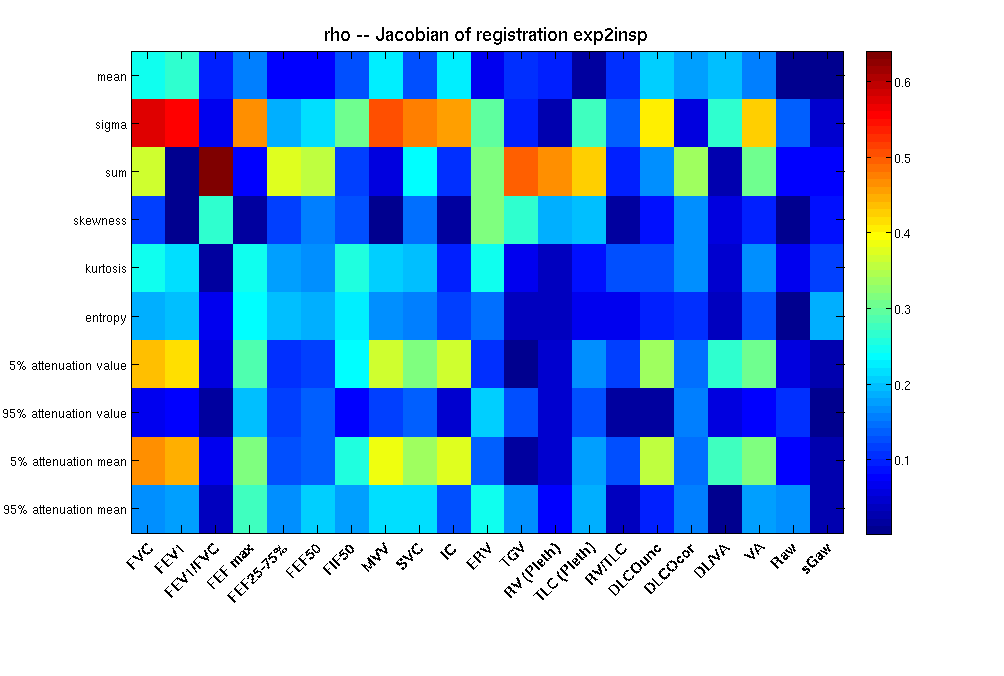
\includegraphics[width=0.9\linewidth,viewport=100 60 620 520]{rho_jac.png}
 \caption{rho\_jac. PFT correlated with Jacobian of lung registration, from expiration to inspiration, rho value.}
\end{figure}

\begin{figure}
 % \centering
 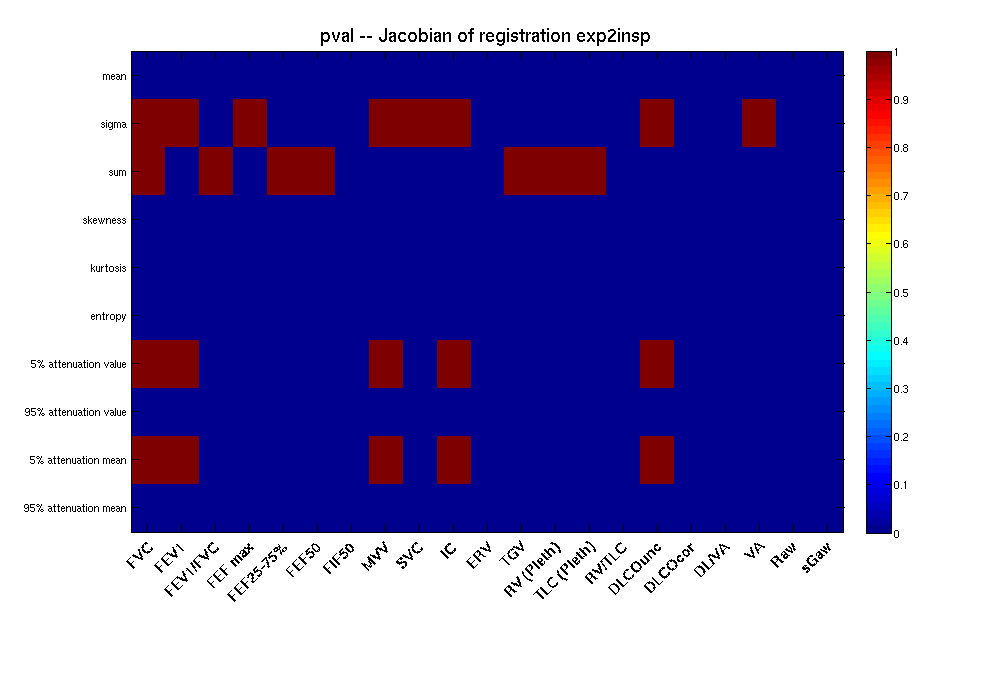
\includegraphics[width=0.9\linewidth,viewport=100 60 620 520]{p_jac.png}
 \caption{p\_jac. PFT correlated with Jacobian of lung registration, from expiration to inspiration, p value $<$ 0.01.}
\end{figure}

\begin{figure}
 % \centering
 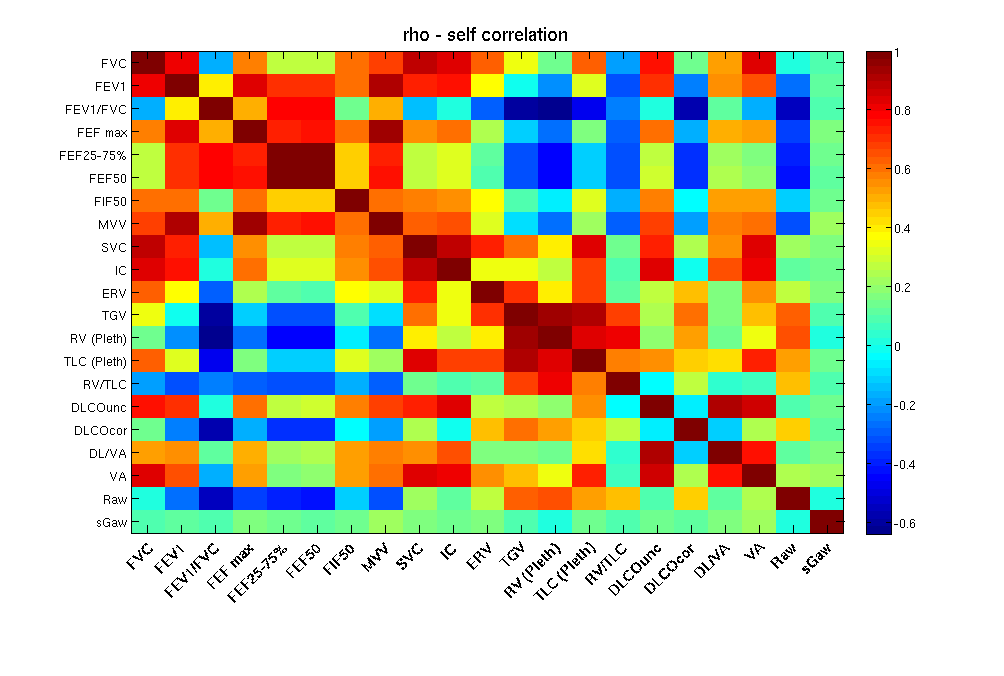
\includegraphics[width=0.9\linewidth,viewport=100 60 620 520]{rho_self.png}
 \caption{rho\_self. PFT correlated with PFT, rho value.}
\end{figure}

\begin{figure}
 % \centering
 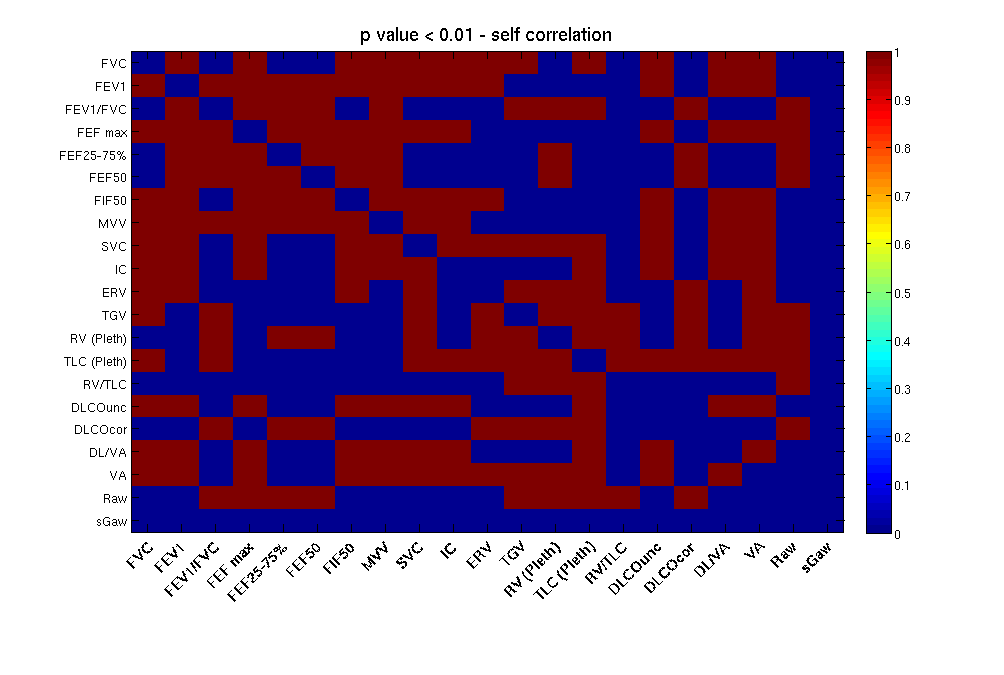
\includegraphics[width=0.9\linewidth,viewport=100 60 620 520]{p_self.png}
 \caption{p\_self. PFT correlated with PFT, p value $<$ 0.01.}
\end{figure}

\end{document}
